\subsection{Tutorien}

In diesem Abschnitt geht es um eure Tutorengruppen, die aus 2 Tutorengruppenleitern (Tutoren) sowie 10--15 Erstis bestehen und euch den Einstieg ins Studium erleichtern sollen.\\
Erfahrungsgem"a"s treten in der Anfangszeit einige Fragen auf. Oft wei"s man noch nicht genau, an wen man sich wenden sollte oder kann den etwas bescheidenen Internetseiten der TU nicht die richtigen Informationen entlocken. In diesen F"allen sind die Tutoren die richtigen Ansprechpartner.\\
Jedem Ersti soll in der Einf"uhrungswoche (s. Termine) eine Tutorengruppe zugeteilt werden. Damit auch ihr wisst, an wen ihr euch wenden k"onnt, solltet ihr diese Einteilung und das anschlie"sende erste Treffen nicht verpassen!\\
Dort habt ihr dann die M"oglichkeit in "uberschaubarer Runde andere Informatikstudenten des 1. Semesters kennen zu lernen, Fragen zu stellen, weitere Informationen zu euren Veranstaltungen und Dozenten zu erhalten und das Campusgel"ande kennen zu lernen.\\
Scheut euch nicht einen der Tutoren zu kontaktieren. Ihr k"onnt euch auch nachtr"aglich noch in eine Tutorengruppe einteilen lassen, da weitere Treffen geplant sind. Dazu schreibt bitte eine Mail an die Fachgruppe fginfo@tu-bs.de oder direkt an einen der Tutoren.\\
Damit ihr auch ein paar Gesichter zuordnen k"onnt - gerade wenn ihr eventuell selbst noch keinen Tutor habt - sind hier Fotos einiger Tutoren abgebildet:

\onecolumn

% \begin{figure}[h]
%   \subfloat[Hella 1\newline h-f.hoffmann@tu-bs.de]{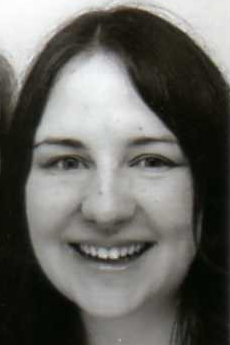
\includegraphics[width=0.45\linewidth]{bilder/tutoren/hella}}
%   \hfill
%   \subfloat[Hella 2]{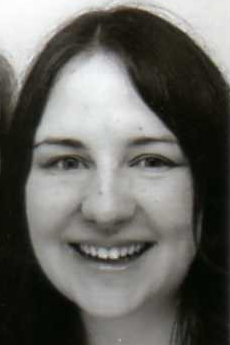
\includegraphics[width=0.45\linewidth]{bilder/tutoren/hella}}
% \end{figure}

\npicture[0.3\linewidth]
{bilder/tutoren/hella}
{Hella\\3. Semester\\h-f.hoffmann@tu-bs.de}
\hfill
\npicture[0.3\linewidth]
{bilder/tutoren/winnie}
{Winnie\\3. Semester\\ ~}
\hfill
\npicture[0.3\linewidth]
{bilder/tutoren/dominik}
{Dominik\\3. Semester\\d.schuermann@tu-bs.de}
\par \ \par
\npicture[0.3\linewidth]
{bilder/tutoren/henning}
{Henning\\7. Semester\\h.guenther@tu-bs.de}
\hfill
\npicture[0.3\linewidth]
{bilder/tutoren/martinw}
{Martin\\7. Semester\\ ~}
\par \ \par

\twocolumn